%%=============================================================================
%% Methodologie
%%=============================================================================

\chapter{Methodologie}
\label{ch:methodologie}

%% TODO: Hoe ben je te werk gegaan? Verdeel je onderzoek in grote fasen, en
%% licht in elke fase toe welke stappen je gevolgd hebt. Verantwoord waarom je
%% op deze manier te werk gegaan bent. Je moet kunnen aantonen dat je de best
%% mogelijke manier toegepast hebt om een antwoord te vinden op de
%% onderzoeksvraag.

\section{Wat zijn de redenen van een omschakeling?}
\label{sec:methodologie-redenen-omschakeling}

TO DO
- slechte monitoring
- slecht geautomatiseert 
- geen multi environment

\section{Technische werking van Ansible en Puppet?}
\label{sec:methodologie-technische-verschillen}

\subsection{Overzicht van Puppet en Ansible}


\begin{tabular}{ r |c c }
&Ansible & Puppet \\
  \hline	  		
Programmeerparadigma\footnote{synoniemen zijn ook programmeerstijl of programmeermodel, voorbeelden zijn object-geori\"onteerd, procedureel, imperatief..., \autocite{journalofinformation} }  & declaratief & declaratief  \\
   \hline
 Programmeertaal &eigen DSL & YAML \\
     \hline
   Communicatieprotocol & SSH & HTTPS \\
   \hline
   open poorten\footnote{Dit is de minimale vereisten van open poorten. Voor sommige features dienen meer poorten open te zijn. Bijvoorbeeld 443 voor Ansible Tower of 8140 op elke Puppetclient voor puppet kick functionaliteit \autocite{puppetkick} }  & 22/tcp (client) & 8140/tcp (master)\\
   
  

  \end{tabular}



 \autocite{languagePuppet}\autocite{masterproef} \autocite{ansibledoc}

\subsection{Werking van Puppet}

Tussen de master en de client bestaat er een vertrouwensrelatie die onderhouden wordt door certificaten. Het is de Puppetmaster die verantwoordelijk is voor het verlenen van deze certificaten. Pas als dit alles in orde is, kan Puppet  aan de configuraties van de clients beginnen. De code die je schrijft wordt een manifest genoemd. Wanneer een Puppetagent wil controleren of hij nog up-to-date is, zal hij een catalogus aanvragen bij de Puppetmaster. Een dergelijke catalogus is in feite een manifest dat de Puppetmaster compileert. Deze catalogus is bovendien uniek voor elke Puppetagent. Dit komt omdat er bij het compileren van het manifest naar de catalogus rekening gehouden wordt met diverse parameters zoals de functie van de server of de distributie van het besturingssysteem dat op die server draait \autocite{Puppetlanguagecatalog}. Eens de Puppetagent zijn persoonlijke catalogus ontvangen heeft, zal deze voor zichzelf controleren of er verschillen zijn tussen zijn huidige configuratie en de staat die beschreven staat in de catalogus. Indien er afwijkingen zijn, worden deze ook automatisch opgelost \autocite{Puppetdoc}.

\subsection{Werking van Ansible}


Ansible maakt geen gebruik van agenten. Dit betekent dat de ansibleserver enkel de naam en het wachtwoord dient te kennen van de servers die hij moet configureren. De verzameling van alle configuraties wordt een playbook genoemd. Het authenticeren kan op verschillende manieren. Er wordt aangeraden om gebruik te maken van een SSH-key, wat het eenvoudigst is, maar ook andere middelen zoals met een eenvoudig wachtwoord of het kerberos-protocol worden ondersteund. Eens de verbinding tot stand is gebracht, verstuurt Ansible modules naar de te configureren server. Deze modules worden vervolgens uitgevoerd en weer verwijderd. Ook Ansible bezit de functionaliteit om na te gaan of de huidige configuratie in lijn is met de ontvangen modules. Om servers te configureren met Ansible bestaan er bovendien twee manieren. Ansible playbooks kunnen in principe verstuurd worden naar de servers vanaf elke computer. Voor een grotere hoeveelheid servers is dit echter niet aangeraden en bestaat er de commerci"ele versie waarbij de playbooks worden verstuurd vanaf een centraal punt. Dit centraal punt is voorzien van Ansible Tower die een inventaris heeft van alle servers en playbooks die onder zijn verantwoordelijkheid vallen \autocite{ansibledoc}.


\subsection{Performantie}
  Time to establisch connection and prepare for configuration \newline
\begin{tabular}{| r |c |c |c |c |c |c |c |c |c |c |c |c |c |c |c |c |c |c |c |c |c |c |c |c |}
  \hline	  		
Puppet & 9 & 6 & 6 & 	11 & 	6 & 7 & 8 & 6 & 9 & 9 & 7 & 7 &	 8 & 6 & 6 & 9 & 10 & 8 & 8 & 7\\
   \hline
  Ansible & 9 & 5 & 5 & 7 & 4 & 5 & 6 & 5 & 4 & 11 & 6 & 4 & 8 & 10 & 7 & 5 & 6 & 4 & 9 & 5 \\
  \hline  
\end{tabular}


Time to configure

\begin{tabular}{| r |c |c |c |c |c |c |c |c |c |c |c |c |c |c |c |c |c |c |c |c | c c |}
  \hline			
  
Puppet & 51,35 & 43,56 & 46,78 & 55,18 & 40,59 & 47,01 & 35,99 & 35,07 & 43,29 & 42,28 & 42,20 \\ \hline
            & 96,83 & 32,33 & 49,99 & 40,32 & 55,62 & 52,82 & 42,72 & 44,21 & 43,13 & &  \\ \hline
            
   
  Ansible & 67 & 60 & 51 & 59 & 51 & 51 & 59 & 57 & 45 & 90 & 52  \\ \hline
                & 53 & 54 & 52 & 62 & 68 & 51 & 59 & 53 & 45 & & \\
  \hline  
\end{tabular}

\subsection{Belasting van het netwerk}

Ansible en Puppet hebben een groot verschil in de manier van communiceren en dit weerspiegeld zicht in het gedrag van de CMT. Op afbeelding \ref{fig:netwerkverbruikpernode} bevinden zich links alle Ansible clients, te herkennen aan hun naam die begint met een A. Rechts staan alle puppet clients, te herkennen aan de PP. De grafieken weerspiegelen uitsluitend het dataverkeer tussen de server (Ansible Tower of Puppetmaster) en de desbetreffende client. Andere data, zoals bijvoorbeeld het downloaden van services of uploaden van logbestanden naar de monitoringstool zijn hierin niet opgenomen. Dit word verwezenlijkt door gebruik te maken van verschillende netwerkkaarten. Wanneer er geen deploy gebeurde was de kilobyte/ minuut op deze netwerkkaart gelijk aan nul, een bewijs dat hier geen andere data dan deze van de CMT over word verstuurd.  \newline

De mannier van communicatie is te herkennen in de grafieken. Zo onderhoud Ansible de communicatie met de client gedurende de deploy. Hiermee wordt bedoelt dat Ansible op de hoogte is van de laatste stand van zaken op de client. Wanneer een bepaalde taak voltooid is wordt Ansibel Tower hier onmiddelijk van op de hoogte gebracht. Op afbeelding \ref{fig:netwerkverbruikpernode} komt deze mannier van werken duidelijk terug op grafiek Anode1 en Anode2. Hier is te zien hoe het netwerk voordurend belast wordt. Ook grafiek Anode3 - Anode5 zijn volgens deze logica te verklaren. Ansible verstuurd namelijk enkel data als de verandering voltooid is. Er worden dus geen onnodige berichten verstuurd. De 'val' in de grafiek Anode3 - Anode5 is dus te verklaren een trage download van een bepaalde service\footnote{Hier betreft het de service MariaDB}. De download duurde langer dan een minuut waardoor er een minuut lang niets te rapporteren viel. Deze mannier van werken is handig tijdens het schrijven van nieuwe Ansible rollen. Je krijgt namelijk live feedback tijdens het uittesten. Een nadeel hieraan is dat het netwerk geen rust krijgt. Bovendien word deze functionaliteit van 'live feedback' in productie niet vaak gebruikt. In realiteit lopen deze jobs tijdens de nacht en is het voldoende om de dag erop een algemeen overzicht te krijgen.\newline

Bij puppet is dit anders. Hierbij is er enkel communicatie tussen de server en de client op het begin en het einde van de deploy. Dit komt duidelijk terug in PPnode1, PPnode4 - PPnode6. Ook grafiek PPnode3 is op deze mannier te verklaren. Hier ging het downloaden van de services namelijk veel vlugger, waardoor na 1 minuut het bericht van voltooid al verstuurd kon worden. Een nadeel hieraan is dat er op de master geen live feedback voor testen gevolgd kan worden. Dit kan echter wel opgelost worden door in te loggen op de client en hier de live feedback volgen met het commando 'puppet agent -t'. Het wordt wel nog steeds pas op het einde van de deploy terug naar de master gestuurd?
 \newline
\textbf{TO DO: wat is dit zogenaamde bericht van voltooid? Worden er bij Puppet wel log files terug naar de master gestuurd? te onderzoek en te vragen aan Pieter}

Vervolgens is er ook gekeken naar de totale netwerkbelasting. Hiervoor is er per client een cumulatie genomen van de kilobytes/minuut gedurende de gehele deploy. Deze waarden zijn terug te vinden in grafiek \ref{fig:netwerkverbruik}. Hier heeft Ansible een gemiddelde van 927,32 kilobytes/deploy en Puppet 1885,9 kilobytes/deploy. Belangrijk om te weten is dat er getracht is geweest het playbook van Ansible en het manifest van Puppet zo gelijkaardig mogelijk te houden. 


\begin{figure}
  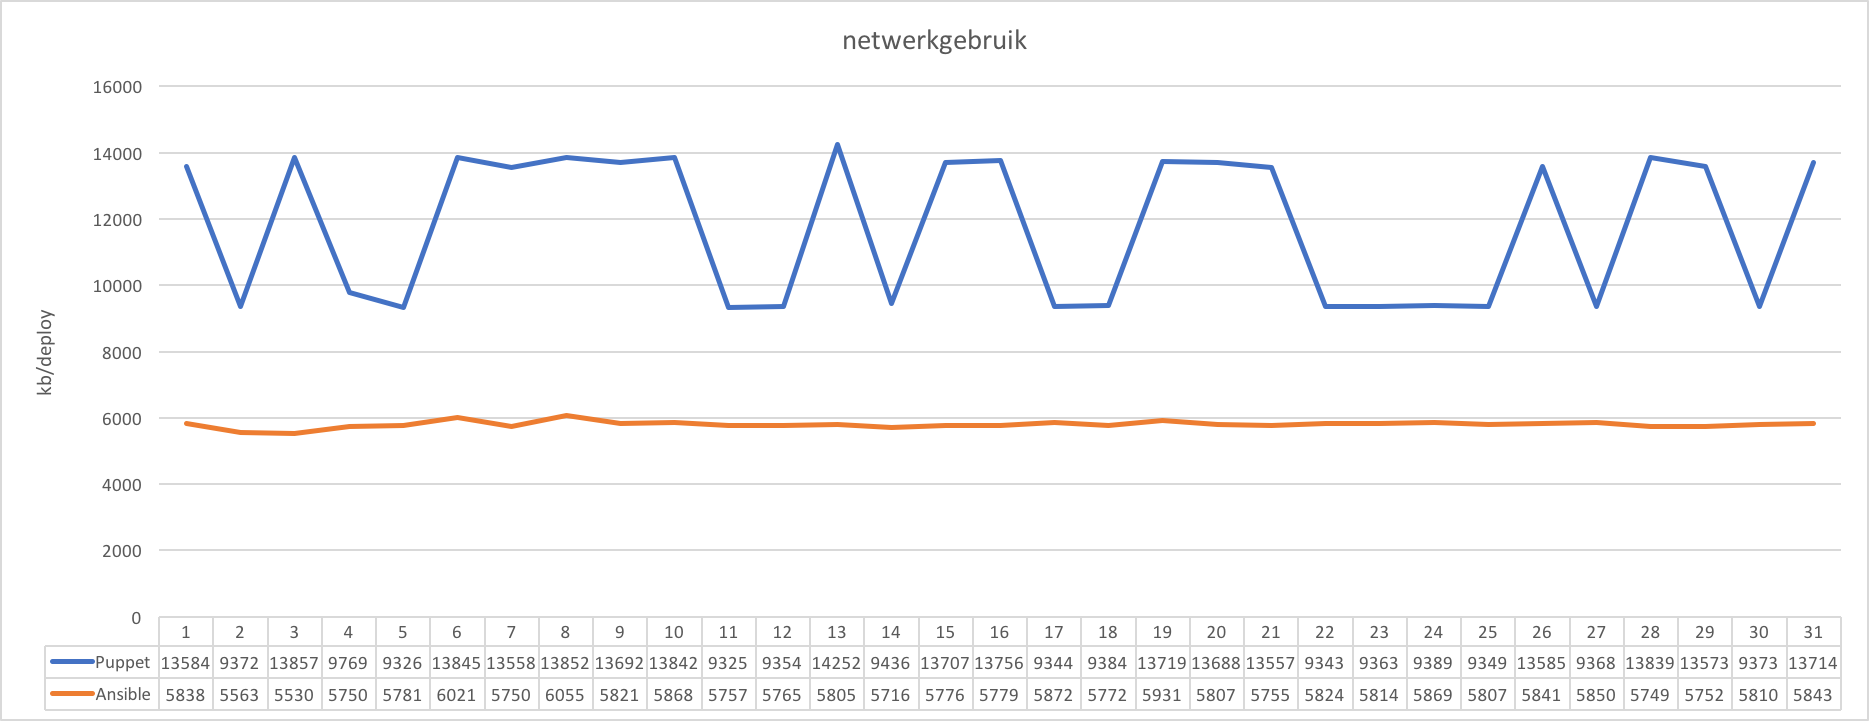
\includegraphics[width=\linewidth]{img/netwerkverbruik.png}
 \caption{Totaal verbruikte netwerkcapaciteit per client gedurende het deployen. Dit bevat enkel communicatie tussen master en client.}  
  \label{fig:netwerkverbruik}
\end{figure}


\begin{figure}
  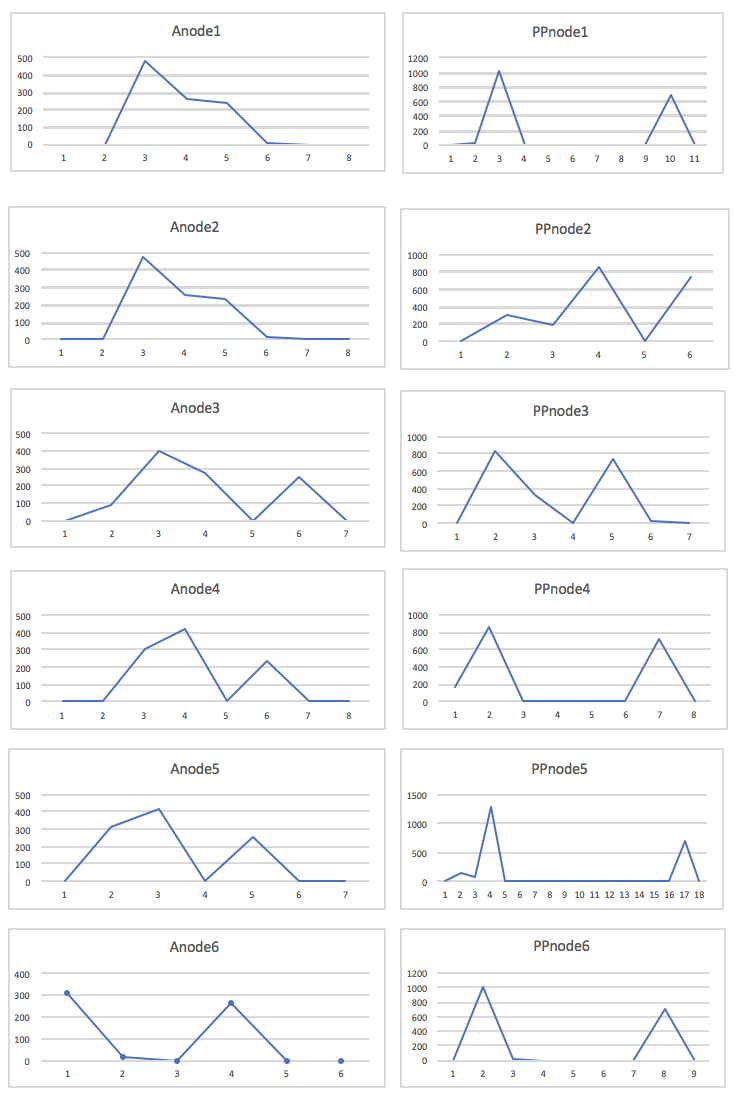
\includegraphics[width=\linewidth]{img/netwerkverbruikpernode.png}
 \caption{Aantal kilobytes per minuut op een netwerkkaart die uitsluitend bedoelt voor communicatie met Ansible Tower / Puppetmaster. }  
  \label{fig:netwerkverbruikpernode}
\end{figure}

\subsection{Gebruik van het geheugen}

Op grafiek \ref{fig:geheugengebruik} is per tijdseenheid het gemiddelde gebruikte ramgeheugen weergegeven. Hierop is te zien hoe Puppet opvallend meer geheugen gebruikt. Niet alleen tijdens een deploy maar ook ervoor en erna. Zelfs wanneer een Ansible client en een Puppet client juist opgezet worden met behulp van de Vagrantfile is er al een verschil in het gebruikte geheugen. Gezien het feit dat er al een verschil waar te nemen is in deze vroege levensfase van de server en het enige verschil in configuratie op dit moment de Puppet agent is werd vermoed dat het verschil hier aan te wijten is. Dit vermoeden werd gestaafd toen de puppet agent tijdelijk uitgezet werd. Het ramgeheugen daalde onmiddelijk naar gelijkwaardige waarden als deze van de Ansible client. Zonder configuratie hebben Puppet clients een gemiddeld verbruik van 47,6\% gebruikt geheugen. Bij Ansible is dit 38,2\%. Dit betekend dat met een verschil van 9,4\% er bij 500 MB, 47MB gebruikt wordt aan Puppet.


\begin{figure}
  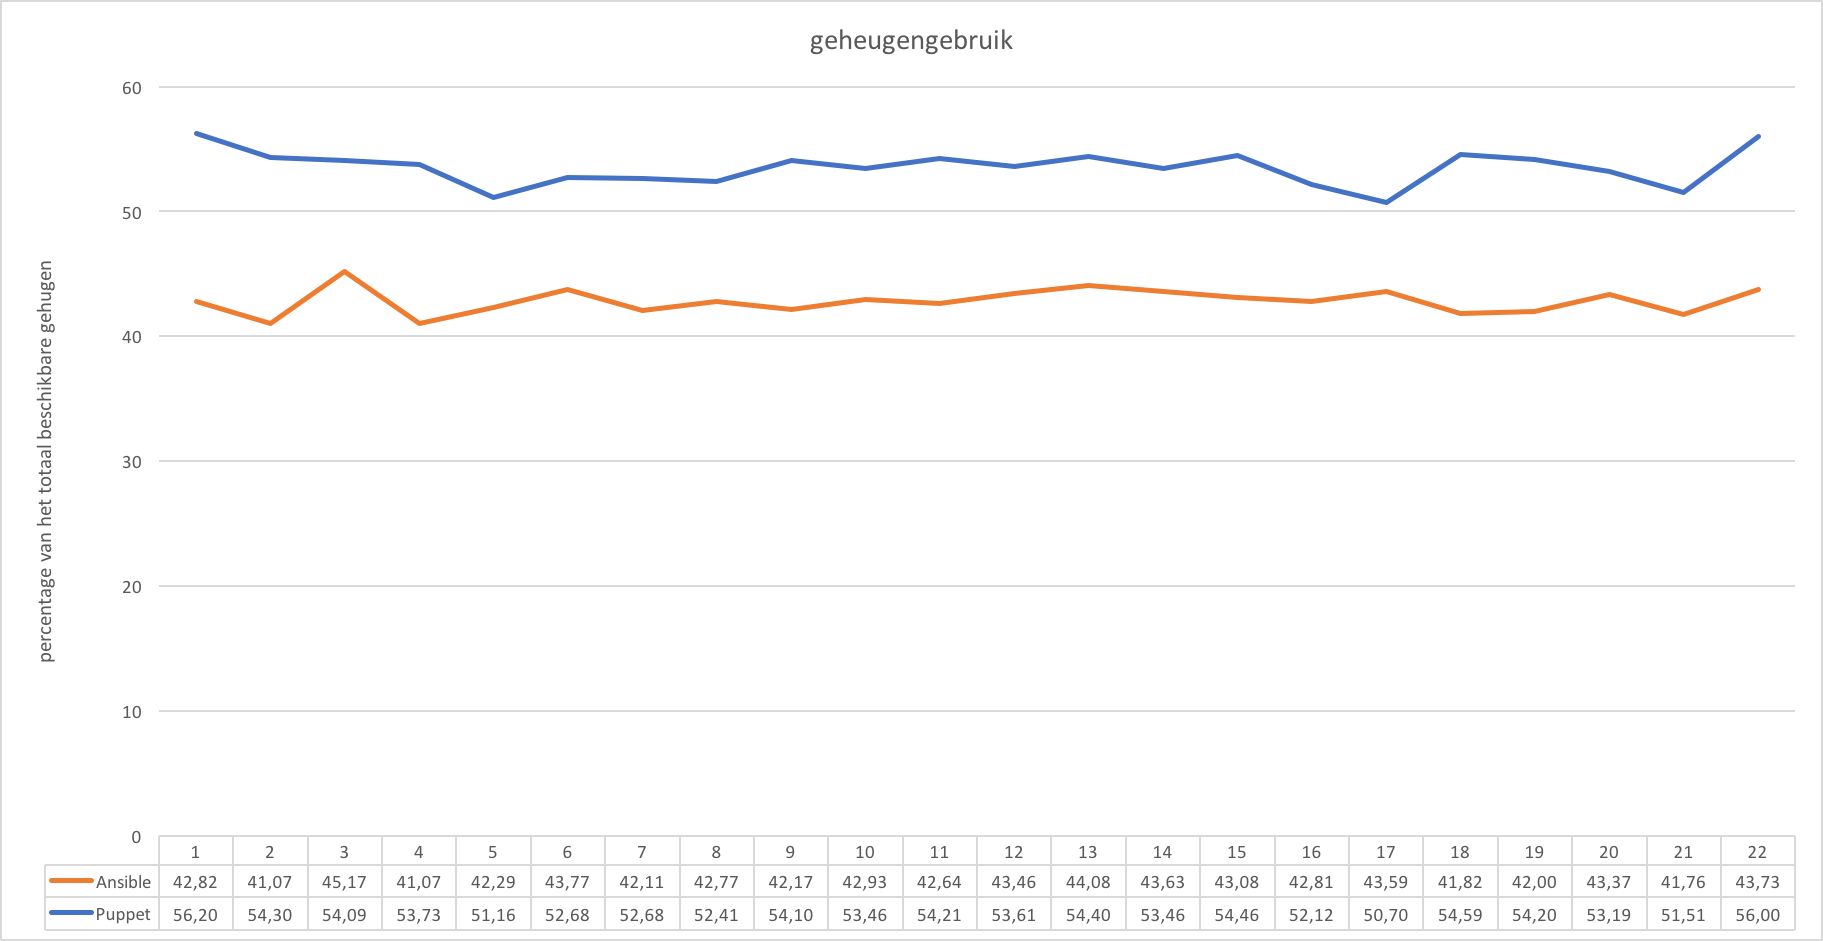
\includegraphics[width=\linewidth]{img/geheugengebruik}
 \caption{Verbruikt percentage van het RAM geheugen. Gemeten bij servers met elk 500 MB. }  
  \label{fig:geheugengebruik}
\end{figure}



\section{Wat is het verloop van een dergelijke transitperiode?}
\label{sec:methodologie-verloop-transit}









